\documentclass[11pt,a4paper]{scrartcl}
\typearea{12}
\usepackage{graphicx}
\usepackage{pstricks}
\usepackage{listings}

\usepackage{tikz}

\usepackage{pgf}
\usepackage[utf8]{inputenc}
\usetikzlibrary{arrows,automata}
\usetikzlibrary{positioning}


\tikzset{
    area/.style={
      circle,
           draw=black, very thick,
           inner sep=2pt,
           text centered,
           },
}


\tikzset{
    center/.style={
      circle,
           draw=black, very thick,
           inner sep=2pt,
           text centered,
           minimum size=2.5cm,
           },
}


\tikzset{
    neuron/.style={
      circle,
           draw=red, very thick,
           inner sep=2pt,
           text centered,
           minimum size=2.5cm,
           },
}


\tikzset{
    applic/.style={
      circle,
           draw=green, very thick,
           inner sep=2pt,
           text centered,
           minimum size=2.5cm,
           },
}





\lstset{language=python}
\pagestyle{headings}
\markright{Computational Neuroscience - course plan}

\begin{document}

\begin{figure}
\begin{center}
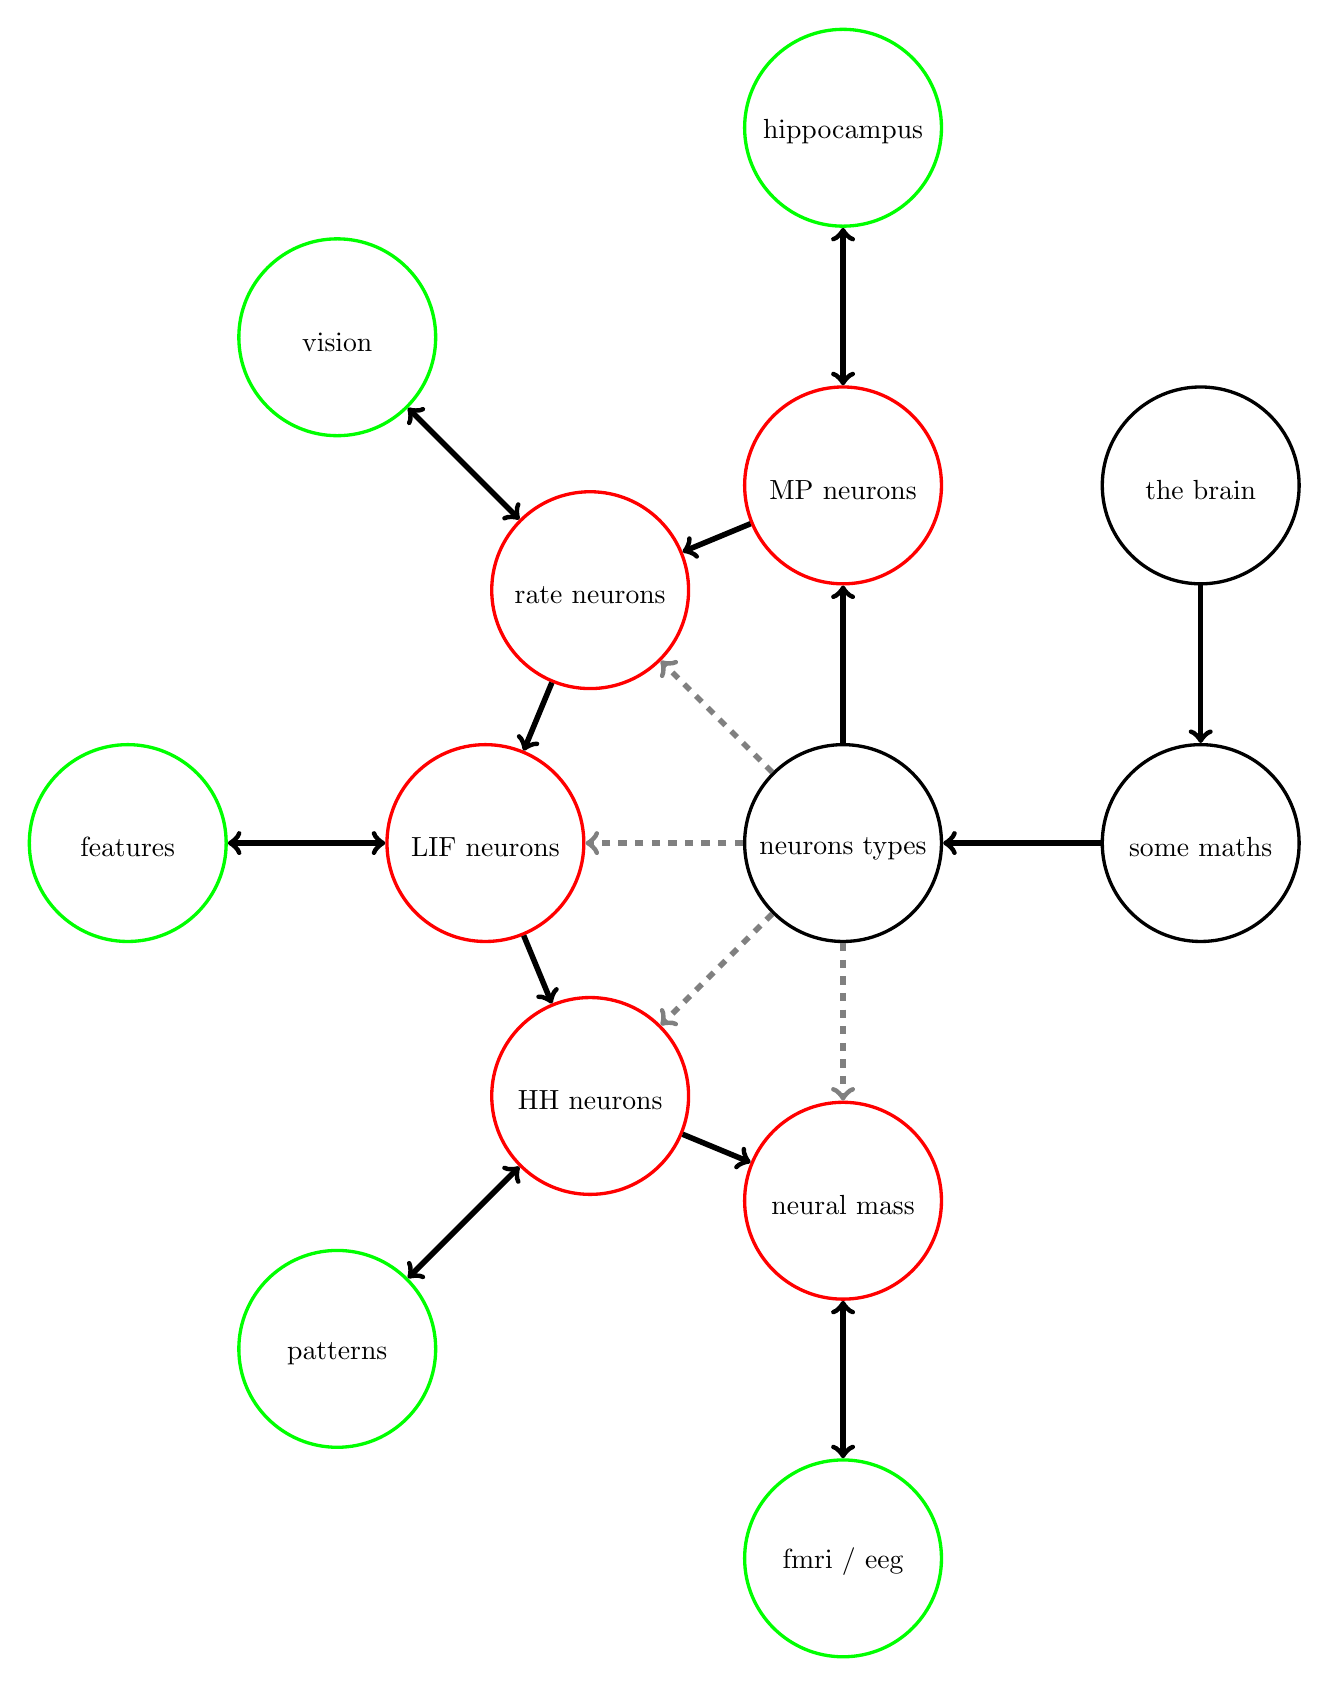
\begin{tikzpicture}

\node[center,text height=0.35cm](nt){neurons types};

\node[center,text height=0.35cm,right = 2cm of nt](sc){some maths};
\node[center,text height=0.35cm,above = 2cm of sc](tb){the brain};


\path (tb) edge[->,line width=2pt](sc);
\path (sc) edge[->,line width=2pt](nt);



\node[neuron,text height=0.35cm,above = 2cm of nt](on){MP neurons};
\node[applic,text height=0.35cm,above = 2cm of on](hpc){hippocampus};

\path (nt) edge[->,line width=2pt](on);
\path (on) edge[<->,line width=2pt](hpc);

\node[neuron,text height=0.35cm,above left = 2cm of nt](rn){rate neurons};
\node[applic,text height=0.35cm,above left = 2cm of rn](vis){vision};

\path (nt) edge[->,line width=2pt,draw=gray,style=dashed](rn);
\path (rn) edge[<->,line width=2pt](vis);


\node[neuron,text height=0.35cm,left = 2cm of nt](ln){LIF neurons};
\node[applic,text height=0.35cm,left = 2cm of ln](pla){features};

\path (nt) edge[->,line width=2pt,draw=gray,style=dashed](ln);
\path (ln) edge[<->,line width=2pt](pla);


\node[neuron,text height=0.35cm,below left = 2cm of nt](hn){HH neurons};
\node[applic,text height=0.35cm,below left = 2cm of hn](pat){patterns};

\path (nt) edge[->,line width=2pt,draw=gray,style=dashed](hn);
\path (hn) edge[<->,line width=2pt](pat);


\node[neuron,text height=0.35cm,below = 2cm of nt](nm){neural mass};
\node[applic,text height=0.35cm,below = 2cm of nm](eeg){fmri / eeg};

\path (nt) edge[->,line width=2pt,draw=gray,style=dashed](nm);
\path (nm) edge[<->,line width=2pt](eeg);

\path (on) edge[->,line width=2pt](rn);
\path (rn) edge[->,line width=2pt](ln);
\path (ln) edge[->,line width=2pt](hn);
\path (hn) edge[->,line width=2pt](nm);


\end{tikzpicture}
\end{center}
\end{figure}

\end{document}
